%! Author = Administrator
%! Date = 2021/7/2

\chapter{详细设计与实现}
基于上一章提出的设计方案,与软件工程的基本原则和设计思想结合,对前端后端通信,后端模块与模块通信,后端与数据层通信的具体业务逻辑实现
以及数据库设计进行了详细的阐述。


\section{架构设计}
由于公有云服务的特殊性,相比较于传统软件系统主要关注功能的可用性,还需要系统做到部署轻便、易维护、高可用、高性能。因此,因此需要更多
的从工程的角度去设计该应用,方便后续的功能添加,业务的扩张扩容,以及代码功能的扩展与维护,这就需要在设计后端架构时,充分考虑到可扩展
性和可维护性,下面将详细阐述使用基于AOP编程思想下的架构设计思路。

采用前后端分离的思想,独立启动前端的页面交互服务守护进程,再通过Nginx将数据层请求转发到后端服务进程,这样一来,后端服务就与前端部分
解耦,可以部署到Docker上作为一个集群提供服务,增强了后期的扩展性。



\subsection{技术方案分析}

根据需求分析的结论,改进点主要有如下:
\begin{enumerate}
    \item 模板服务:提供工作流管理服务,增加应用模板功能。改进业务流程,缓存执行记录表
    \item 调度器服务:提供执行任务时的容器调度,执行记录生成投递等功能。改进容器选择的策略,容器注册心跳检查等功能。
    \item 鉴权服务:提供统一的权限检查。增加缓存层,缓存用户临时Token等数据。
    \item 执行器服务:提供任务执行,容器管理,任务分发等功能,增加预测执行器功能。提供健康检查接口,供调度器可以实时获取每个执行器的信息。
    \item 预测器服务:负责执行记录统计归档,生成任务预测值。
\end{enumerate}


\subsection{模板微服务模块的设计与实现}



\subsubsection{模块设计}



\begin{figure}[H]
    \centering
    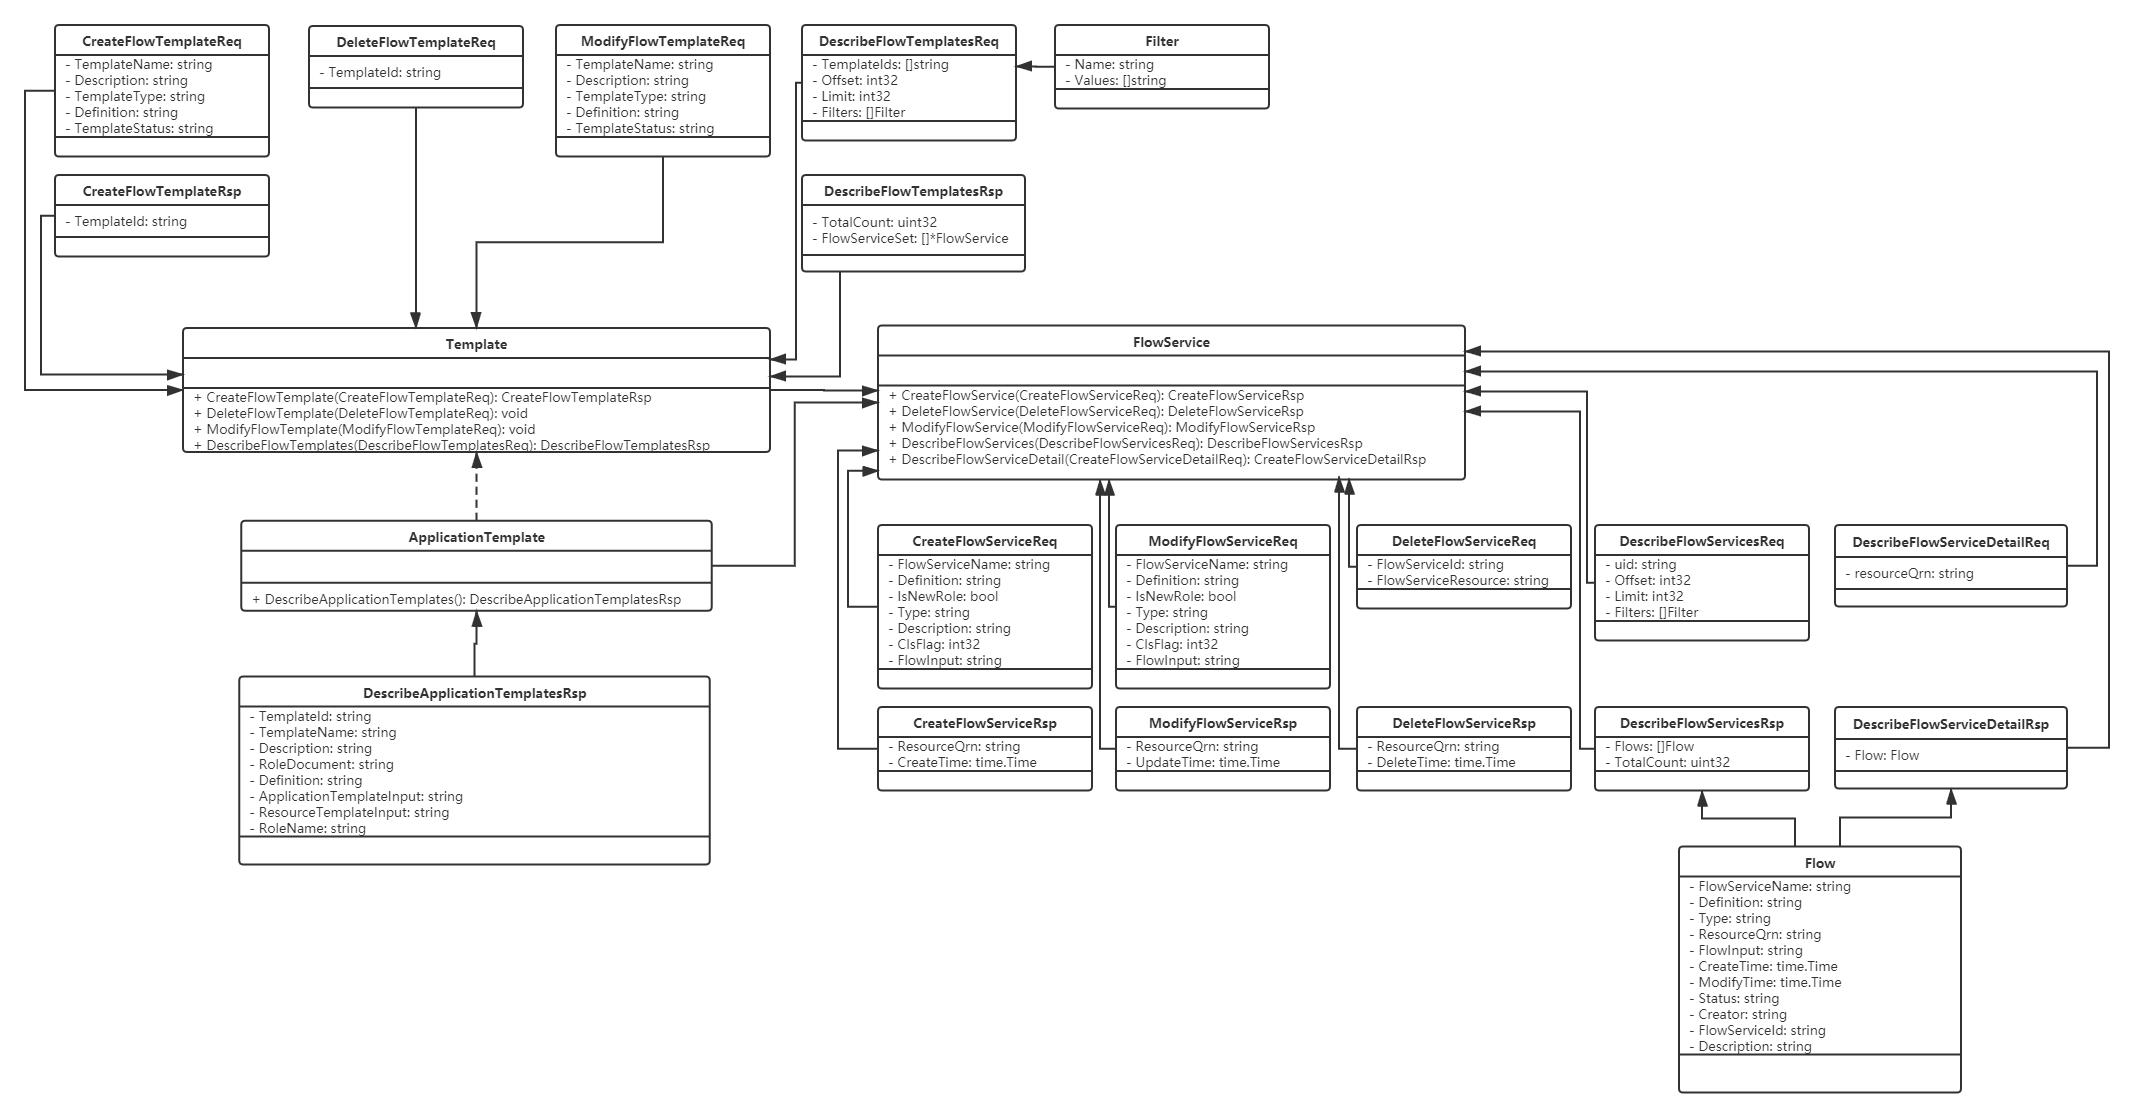
\includegraphics[width=1.0\textwidth]{class-template.png}
    \caption{模板服务类图}
    \label{fig:模板服务类图}
\end{figure}
如图所示,模板服务主要提供工作流与工作流模板的使用服务,工作流模板是一种复杂的工作流,一个工作流模板加上用户提供的参数信息,可以生成一个属于该
用户的工作流。FlowService对象是整个模板服务对外输出的产品,由用户定义的TCSL,或是系统预设的模板、应用模板经由业务逻辑转换而来。
工作流应用模板是一种实际落地场景的解决方案,可以根据不同用户的定制需要,直接实现不同场景下的业务流程。根据应用模板创建工作流时,可以直接生成
工作流对象,开箱即用。
为了提高系统的易用性,系统可以根据创建工作流使用的模板不同,给出样例输入,以及会预先经由工作流执行服务先执行资源创建工作流,为用户工作流中
所涉及的云服务申请权限。再为用户创建工作流。这样,在用户执行时,就不会因为权限问题而抛出错误。




\subsubsection{复杂结构体定义}

\begin{table}[H]
    \centering
    \caption{Template对象定义}
    \label{tab:strcut-template}
    \begin{tabular}{lll}
        \toprule
        字段 & 类型 & 描述 \\
        \midrule
        TemplateId & string & 模板ID \\
        TemplateId &          string& \\
        TemplateName &        string& \\
        Description   &       string& \\
        TemplateCategory  &   string& \\
        TemplateType     &    string& \\
        TemplateStatus    &   string& \\
        CreateDate        &   string& \\
        ModifyDate        &   string& \\
        Creator           &   string& \\
        Modifier          &   string& \\
        Definition        &   string& \\
        ComponentSet      &   []string& \\
        Version           &   int32& \\
        Online            &   string& \\
        Config            &   string& \\
        \bottomrule
    \end{tabular}
\end{table}


\begin{table}[H]
    \centering
    \caption{Flow对象定义}
    \label{tab:strcut-template}
    \begin{tabular}{lll}
        \toprule
        字段 & 类型 & 描述 \\
        \midrule
        FlowId &       string & 工作流ID \\
        FlowName &       string & \\
        Status &                string & \\
        Definition &            string & \\
        RoleResource &          string & \\
        Type &                  string & \\
        CreateDate &            string & \\
        Description &           string & \\
        FlowServiceChineseName & string & \\
        EnableCLS &             bool & \\
        CLSUrl &                string & \\
        FlowInput &             string & \\
        \bottomrule
    \end{tabular}
\end{table}

\subsubsection{接口设计}

模板服务的路由前缀/v1/template/所包含的接口如下:
CreateTemplate
\begin{table}[H]
    \centering
    \caption{创建模板}
    \label{tab:design-interface-template-create}
    \begin{tabular}{llll}
        \toprule
        req, rsp   & 字段 & 类型 & 描述 \\
        \midrule
        req & Template & Template & 待创建的模板对象 \\ \hline
        rsp & TemplateId & string & 创建时生成的模板ID\\
        \bottomrule
    \end{tabular}
    \note{注:}
\end{table}

ModifyTemplate
\begin{table}[H]
    \centering
    \caption{更新模板}
    \label{tab:design-interface-template-modify}
    \begin{tabular}{llll}
        \toprule
        req, rsp   & 字段 & 类型 & 描述 \\
        \midrule
        req & Template & Template & 待删除的模板对象 \\ \hline
        rsp & & & \\
        \bottomrule
    \end{tabular}
    \note{注:}
\end{table}

DeleteTemplate
\begin{table}[H]
    \centering
    \caption{删除模板}
    \label{tab:design-interface-template-delete}
    \begin{tabular}{llll}
        \toprule
        req, rsp   & 字段 & 类型 & 描述 \\
        \midrule
        req & TemplateId & string & 待删除的模板ID(两者只需一个) \\
        & ResourceQrn & string & 待删除的模板Qrn(两者只需一个) \\ \hline
        rsp & & & \\
        \bottomrule
    \end{tabular}
    \note{注:}
\end{table}

CreateFlowService
\begin{table}[H]
    \centering
    \caption{创建工作流}
    \label{tab:design-interface-flow-create}
    \begin{tabular}{llll}
        \toprule
        req, rsp   & 字段 & 类型 & 描述 \\
        \midrule
        req & Flow & Flow & 待创建的工作流对象 \\ \hline
        rsp & ResourceQrn & string & 创建生成的工作流资源Qrn \\
        & CreateTime & time.Time & 工作流创建时间 \\
        \bottomrule
    \end{tabular}
    \note{注:}
\end{table}

ModifyFlowService
\begin{table}[H]
    \centering
    \caption{更新工作流}
    \label{tab:design-interface-flow-modify}
    \begin{tabular}{llll}
        \toprule
        req, rsp   & 字段 & 类型 & 描述 \\
        \midrule
        req & Flow & Flow & 待更新的工作流对象 \\ \hline
        rsp & ResourceQrn & string & 更新的工作流资源Qrn \\
        & UpdateTime & time.Time & 更新时间 \\
        \bottomrule
    \end{tabular}
    \note{注:}
\end{table}


DeleteFlowService
\begin{table}[H]
    \centering
    \caption{删除工作流}
    \label{tab:design-interface-flow-delete}
    \begin{tabular}{llll}
        \toprule
        req, rsp   & 字段 & 类型 & 描述 \\
        \midrule
        req & FlowId & []string & 待删除的工作流ID(两者只需一个) \\
        & ResourceQrn & []string & 待删除的工作流资源Qrn(两者只需一个) \\ \hline
        rsp & ResourceQrn & string & 删除的工作流资源Qrn \\
        & DeleteTime & time.Time & 删除时间 \\
        \bottomrule
    \end{tabular}
    \note{注:}
\end{table}
DescribeFlowServices
\begin{table}[H]
    \centering
    \caption{获取用户名下所有工作流}
    \label{tab:design-interface-flow-services}
    \begin{tabular}{llll}
        \toprule
        req, rsp   & 字段 & 类型 & 描述 \\
        \midrule
        req & uid & string & 需要查询的用户ID \\ \hline
        rsp & Flows & []Flow & 查询到的工作流列表 \\
        & TotalCount & int32 & 查询到的工作流数量 \\
        \bottomrule
    \end{tabular}
    \note{注:}
\end{table}

DescribeFlowServiceDetail
\begin{table}[H]
    \centering
    \caption{获取指定工作流的详情}
    \label{tab:design-interface-flow-detail}
    \begin{tabular}{llll}
        \toprule
        req, rsp   & 字段 & 类型 & 描述 \\
        \midrule
        req & ResourceQrn & string & 待查询的工作流资源Qrn \\ \hline
        rsp & Flow & Flow & 查询到的工作流 \\
        \bottomrule
    \end{tabular}
    \note{注:}
\end{table}


DescribeTemplates:调用该接口以获取指定的模板。
\begin{table}[H]
    \centering
    \caption{查找模板ID对应的模板}
    \label{tab:design-interface-template}
    \begin{tabular}{llll}
        \toprule
        req, rsp   & 字段 & 类型 & 描述 \\
        \midrule
        req & TemplateIds & []string & 待查询的模板templateID \\ \hline
        rsp & Templates & []Template & 查询到的模板信息列表 \\
        & TotalCount & int32 & 查询到的模板数量 \\
        \bottomrule
    \end{tabular}
    \note{注:模板表的}
\end{table}


DescribeApplicationTemplates:调用该接口以获取所有应用模板,通过返回的应用模板相关信息,供前端展示,以及在创建以应用模板为参照的工作流时,
可以通过该接口去获取应用模板ID、资源申请地址、创建所需的资源申请文档以及模板的TCSL定义。
\begin{table}[H]
    \centering
    \caption{显示所有应用模板}
    \label{tab:design-interface-app-template}
    \begin{tabular}{llll}
        \toprule
        req, rsp   & 字段 & 类型 & 描述 \\
        \midrule
        req &&&\\ \hline
        rsp & Id & string & 模板templateID\\
        & Name & string & 模板名称\\
        & Desc & string & 模板描述\\
        & RoleDocument & string & 创建角色需要使用的策略文档\\
        & Definition & string & 模板代码\\
        & ApplicationTemplateInput & string & 应用模板输入\\
        & ResourceTemplateInput & string & 资源创建模板输入\\
        & PolicyDocument & string & 策略文档\\
        & TemplateDetailURL & string & 模板详情页URL\\
        & RoleName & string & 角色名,格式:ASWAppRole-\{12位随机字符串\}\\
        & PolicyName & string & 策略名,格式:ASWAppPolicy-\{12位随机字符串\}\\

        \bottomrule
    \end{tabular}
    \note{注:模板表的}
\end{table}


DescribeTemplateResources:由于云服务的特殊性,并且本系统涉及到多方资源的分配和调用,因此,需要对工作流运行涉及的资源进行统一的管理。
调用该接口以获取该应用模板所需的资源,前端以该接口返回的数据为用户申请资源,对于用户暂未开通,无法自动申请的资源,
根据ServiceUrl,引导用户到相应的云服务控制台处开通该资源。
\begin{table}[H]
    \centering
    \caption{显示部署资源工作流依赖的资源}
    \label{tab:design-interface-resources}
    \begin{tabular}{llll}
        \toprule
        req, rsp   & 字段 & 类型 & 描述 \\
        \midrule
        req & Id & string & 模板templateID\\ \hline
        rsp & Name & string & 模板名称\\
        & Type & string & 资源类型,如云函数、cos桶、cfs文件系统等(1)\\
        & Name & string & 资源名称\\
        & Description & string & 资源描述\\
        & ServiceUrl & string & 服务控制台开通地址\\
        & DescribeStatusUrl & string & 资源状态查询地址(2)\\
        \bottomrule
    \end{tabular}
    \note{注(1):type取值\{api, custom\},api:走api请求;custom:直接打开Action字段对应的网页
    注(2):格式:type | serviceType | inputParams | Action,例:
    API | https://cdn.tencentcloudapi.com | {“Version”: "2017-03-12"} | DescribeClassicLinkInstances
    custom | cos | {} | https://console.cloud.tencent.com/cos5
    }
\end{table}

DescribeDeployResults:获取根据应用模板创建工作流的结果,可以通过轮询的方式来查询此次创建过程是否成功,返回的结果中如果没有一项资源是creating,
则代表可以终止此次轮询以返回最终的结果。
\begin{table}[H]
    \centering
    \caption{查询部署结果}
    \label{tab:design-interface-deploy-results}
    \begin{tabular}{llll}
        \toprule
        req, rsp   & 字段 & 类型 & 描述 \\
        \midrule
        req & ExecutionQRN & string & 此次执行Qrn\\ \hline
        rsp & DeployResults.Id & int64 & 资源主键ID\\
        & DeployResults.DeployResult & string & 部署结果(1)\\
        \bottomrule
    \end{tabular}
    \note{注(1): success: 资源创建成功; failed: 资源创建异常; creating: 正在创建;}
\end{table}


\subsection{调度器微服务模块的设计与实现}


\subsubsection{模块业务流程}

\begin{figure}[H]
    \centering
    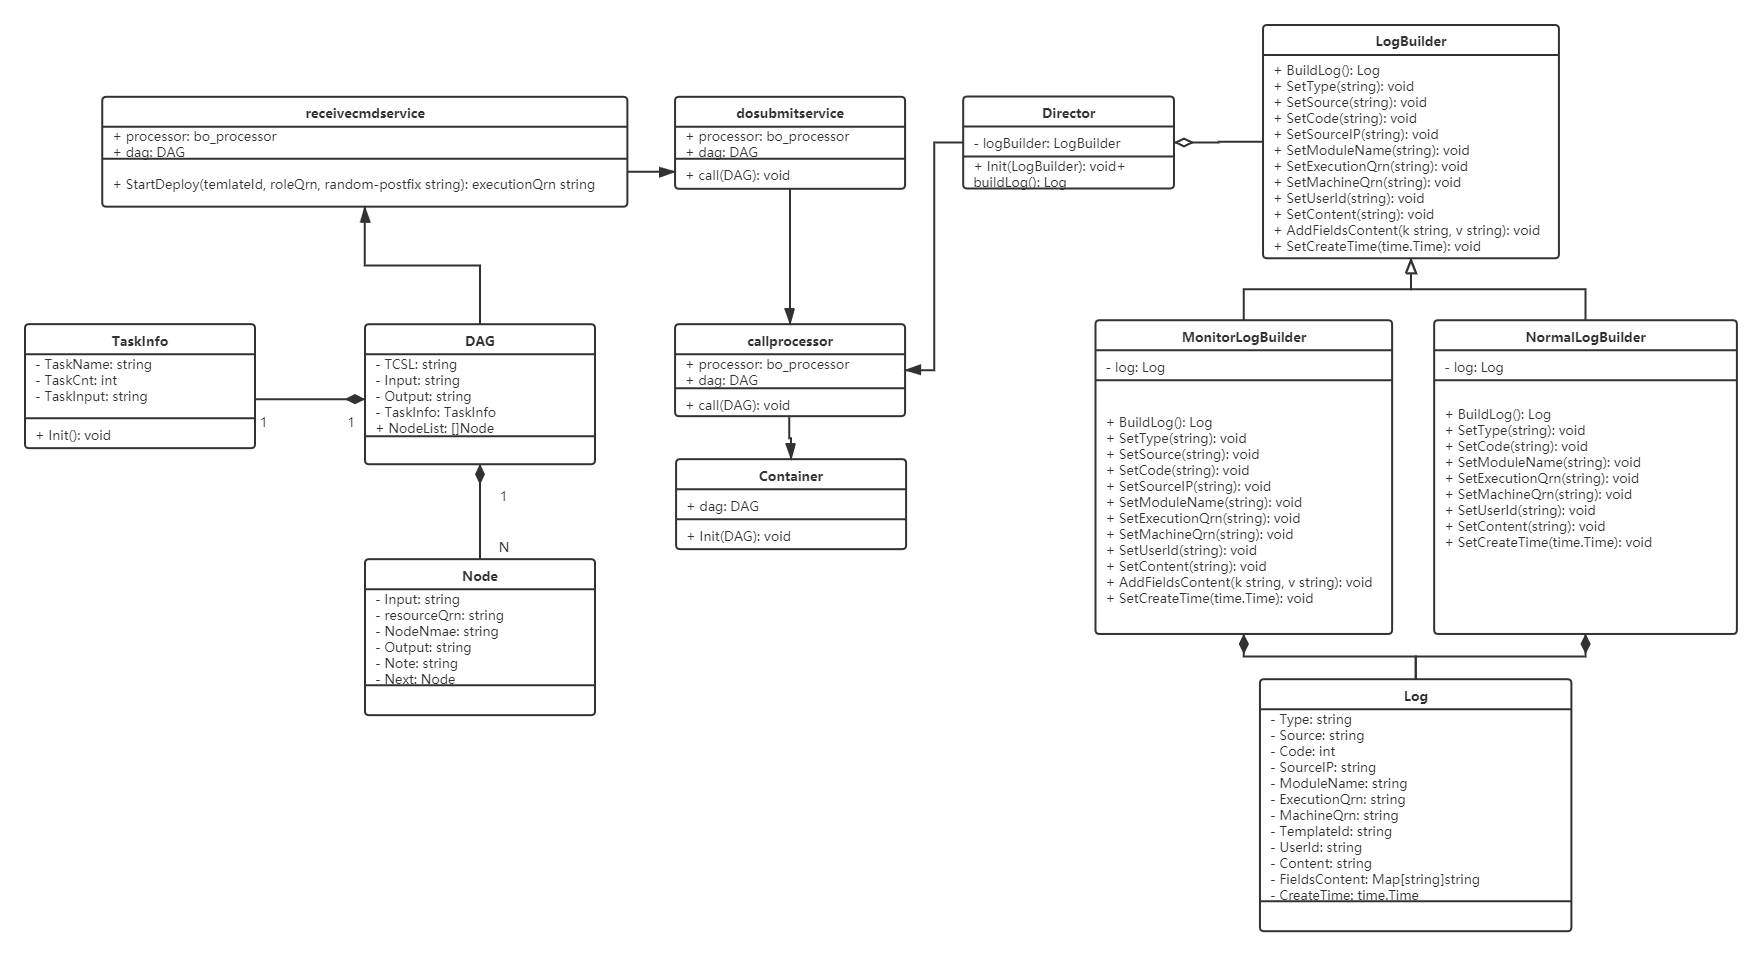
\includegraphics[width=1.0\textwidth]{class-scheduler.png}
    \caption{调度器类图}
    \label{fig:ddqlt}
\end{figure}
该模板负责完成用户提交的任务转化为DAG对象,并将该对象通过特定的路由选择算法发送到执行容器之中执行。如图5-1所示,DAG对象描述一个具体
的任务,里面的TaskInfo字段存储DAG的配置信息,NodeList则存储该DAG所包含的所有任务节点。

调度器模块需要根据执行的结果不同,生成不同的日志。由于其符合建造者模式的思想,因此,将由建造者模式抽象出一个Builder抽象类,该对象支持
构建监控日志、普通日志。前者用于接入云监控系统所需要进行的上报日志,后者用于系统内部的执行日志和用户日志。


该模块设计的目的是保证系统的可扩展性和可维护性。 通过抽象业务场景,以支持较好的可扩展性;保障系统可用性,提高系统的可维护性。

调度器服务的核心能力是将不同类型的用户请求发给合适的执行器。 在这个过程中,调度器应该要肩负这两个重任:
1.抽象任务类型,让系统可以支持更多类型的场景。要支持多种类型的任务,需要做较高层次的抽象,处理数据异构
2.保障系统可用性。要覆盖所有异常情况

2)命令提交

\begin{figure}[H]
    \centering
    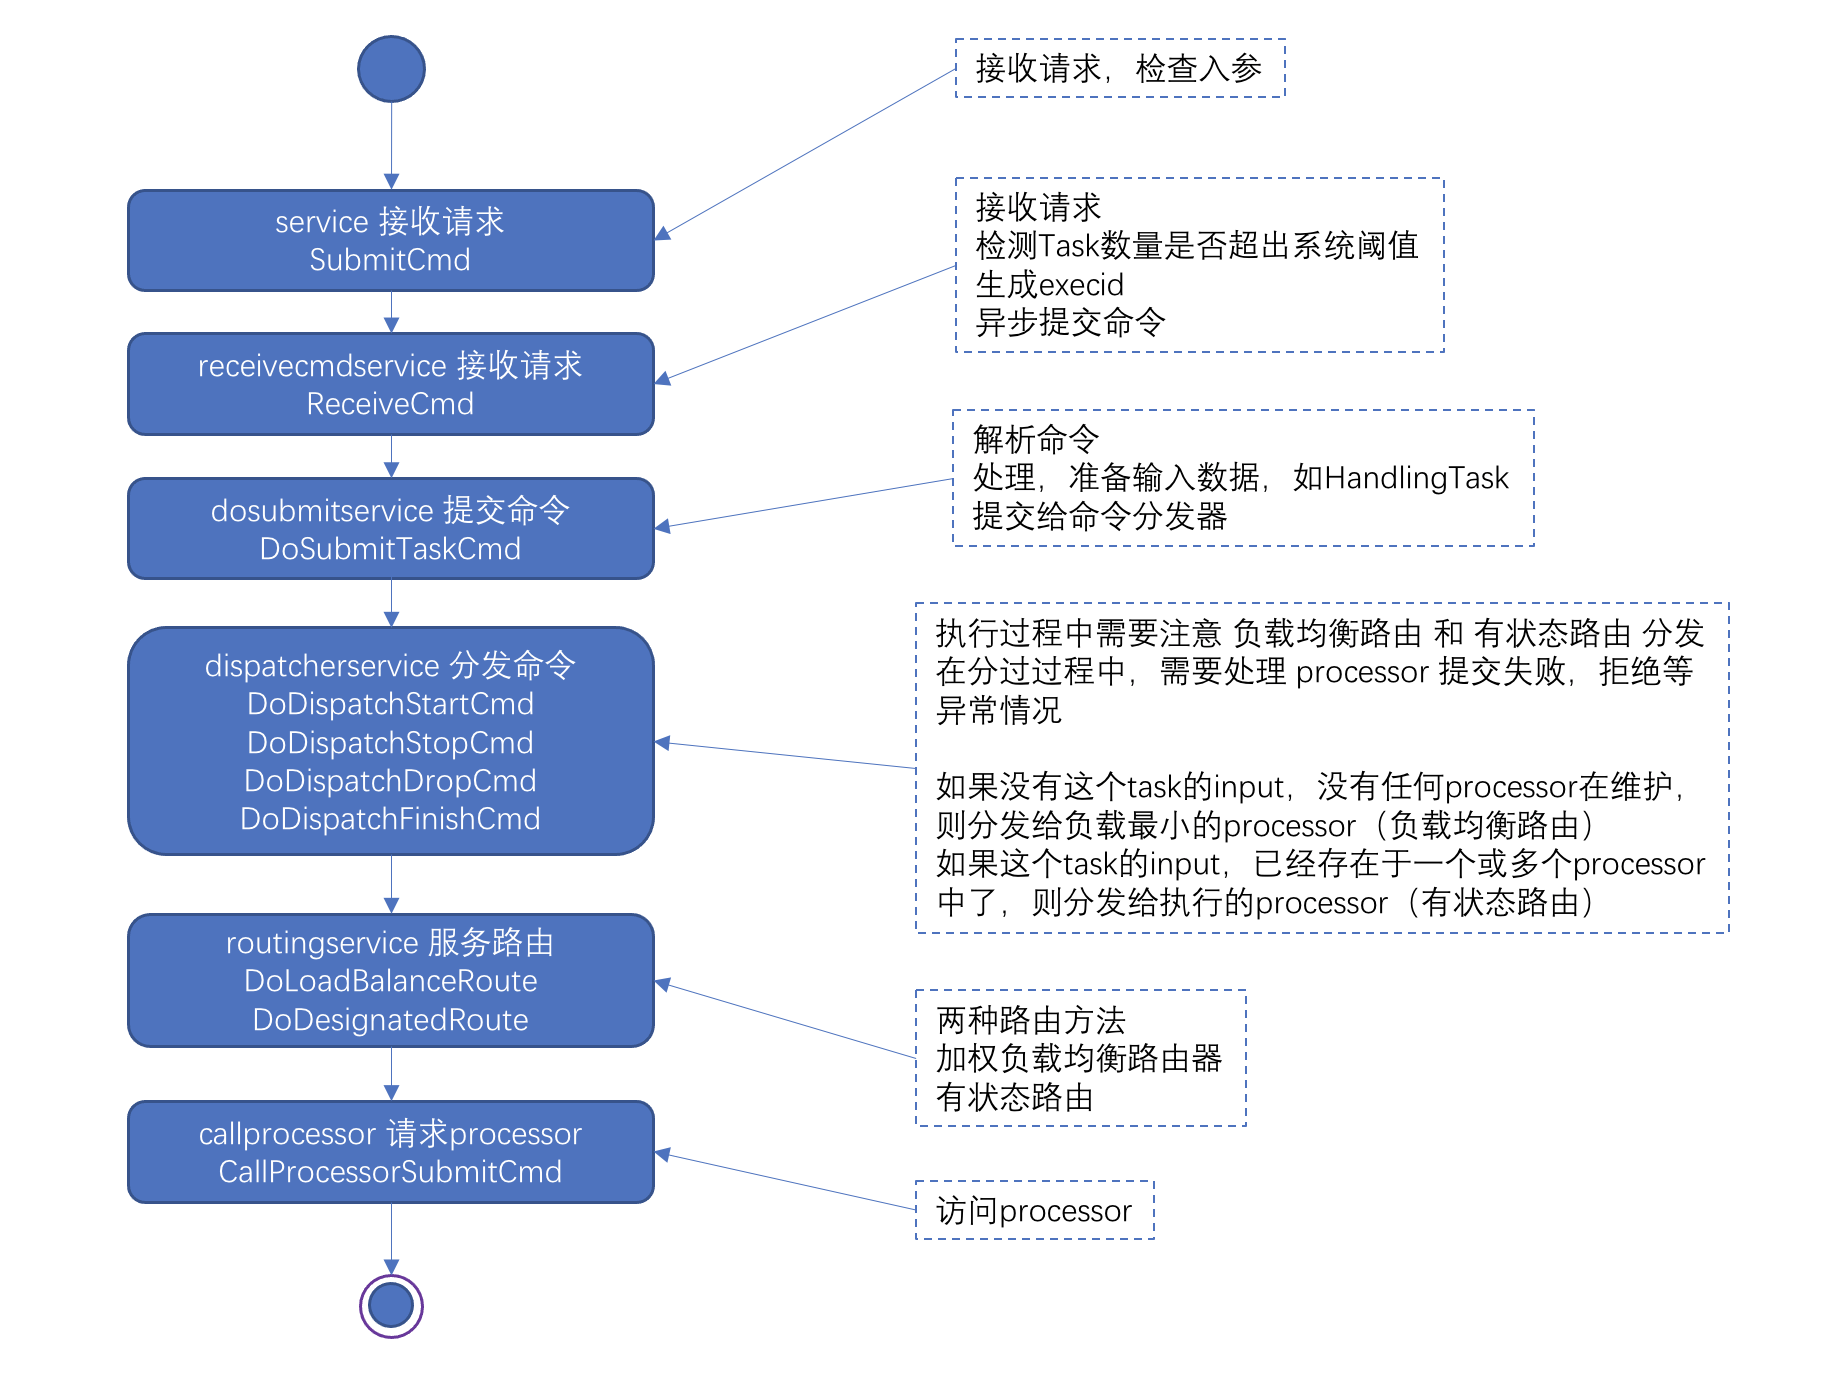
\includegraphics[width=1.0\textwidth]{5-1-1.png}
    \caption{调度器流程}
    \label{fig:调度器流程}
\end{figure}

命令提交是调度器的核心流程,

service层收到请求,进行入参检查,然后调用receiveCmdService处理接收请求逻辑;
receiveCmdService会判断当前系统task的数量,生成执行id,然后启动一个协程来异步提交命令;
doSubmitService 会进行命令的解析,看是哪种命令,来做数据的处理和准备,然后进行命令分发,有分发四种命令,通过相应的逻辑,判断应该用哪种路由,
调用指定的路由方法,调用 callProcessor 打给指定的执行器
callProcessor 执行RPC命令打给指定的执行器;


\begin{figure}[H]
    \centering
    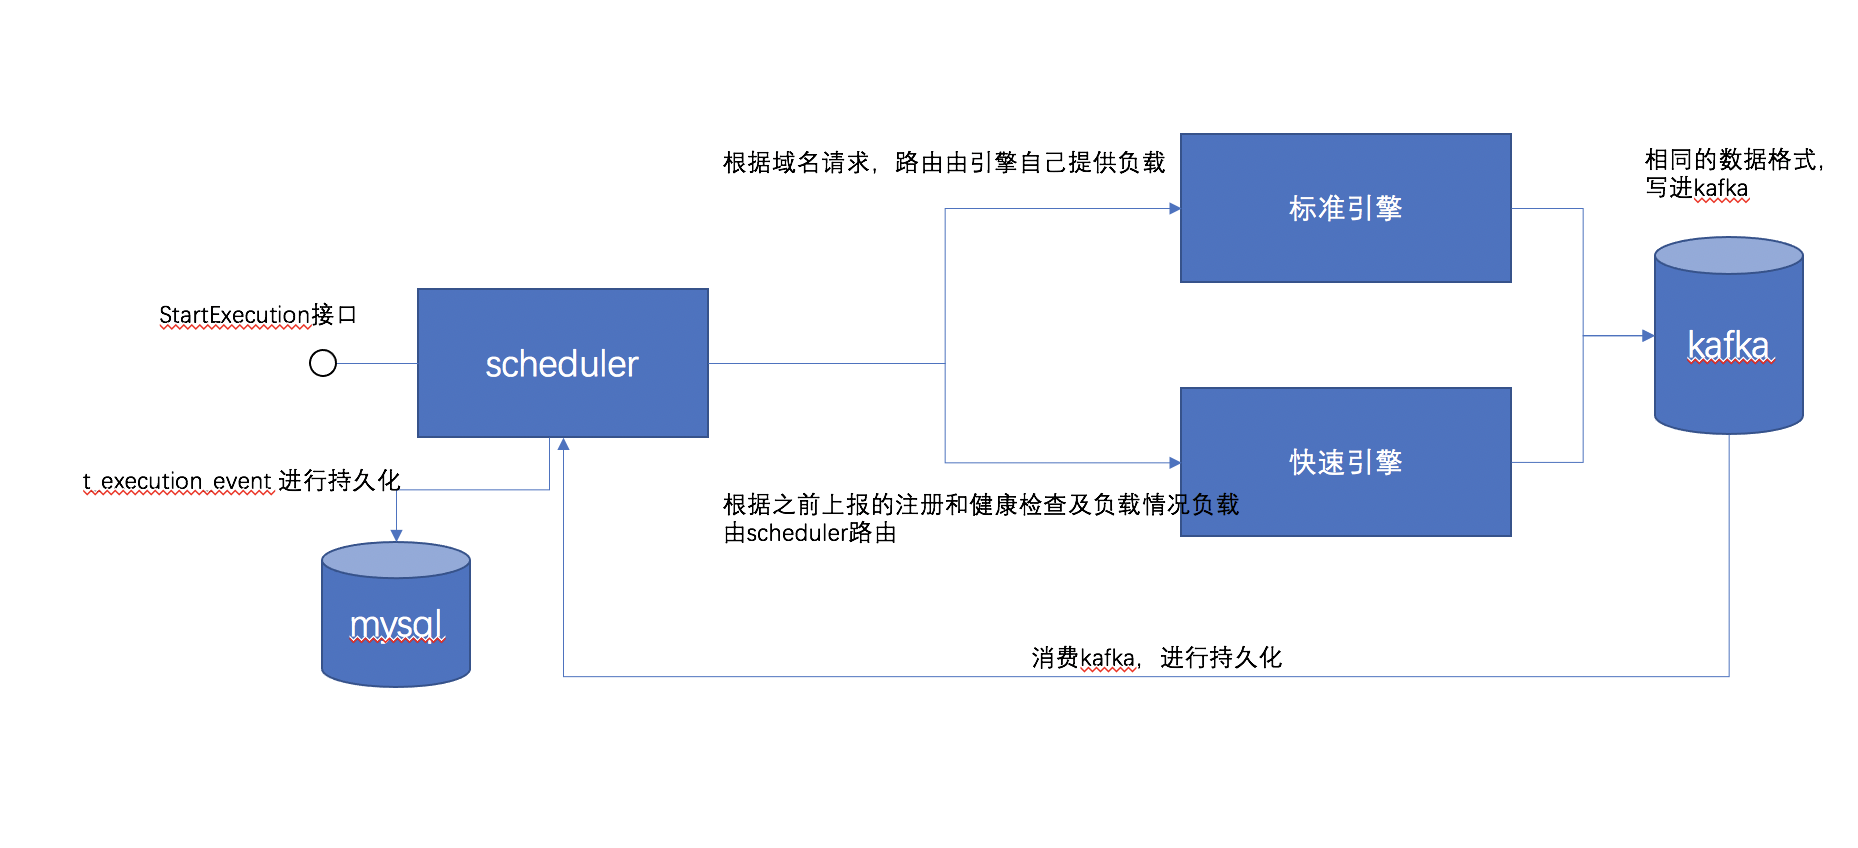
\includegraphics[width=1.0\textwidth]{start-execution-2.png}
    \caption{startExecution数据流转}
    \label{fig:startExecution数据流转}
    \note{}
\end{figure}

startExecution执行过程:

step1 检查这个工作流的状态

step2 先将工作流的状态修改成SCHEDULING

step3 处理任务,从工作流的输入中,检查任务是否以及创建完毕

step4 获取这个任务的所有任务节点

step5 找到目前的任务节点运行的执行容器IP

step6 执行任务分发

step7 将flow的状态修改成RUNNING

概率负载均衡策略:

执行加权负载均衡路由DoLoadBalanceRoute方法

执行负载均衡路由时,如果直接选择简单地直接打给负载最小的 processor,会造成同时打多个请求给一个 processor。反而是不对的。

所以这里对所有执行容器都进行加权平均,然后来选择

之所以不能直接打给负载最小的执行容器。根源是执行容器的负载不是实时的。假设一个工作流有100个任务需要路由分发到执行容器,执行节点的负载值是由心跳
健康检查更新的,不是实时更新的,纯粹按照简单的选择最小的逻辑,会将100个任务同时打给同一个容器。所以,这个复载均衡的策略应该是按照概率打给容器。

概率策略如下:

(公式)对每个任务i p = (100-pi) / sum j∈[0,len), (100-pj),
设4个执行器的负载为pa, pb, pc, pd,
则对于执行器A来说,被选为目标的概率是(100-pa) / (100-pa) + (100-pb) + (100-pc) + (100-pd),
4个processor A,B,C,D的当前负载分别是 10,20,30,40,
则这100个task,打给A的概率是(100-10)/(100-10)+(100-20)+(100-30)+(100-40),
得到概率后,由随机数来决定最终目标。

3)异常流检查和处理

用于处理异常流程的,主要是两个定时器,healthyTimer 和 restartTimer
healthyTimer 用于对容器实例的健康检查
restartTimer 用于对所有非正常任务进行重启

timer 用于定时,timer 到了指定时间会启动 timer 对应的 timerTask。timerTask 执行指定的逻辑。
这些逻辑都是保护逻辑,保护逻辑是不需要所有调度器实例都去执行\cite{jyfw}。

需要引入分布式锁来确保同时只有一个实例在执行timerTask。

比如一到 12:00,进行所有容器实例的健康检查。这个任务,1个调度器去执行就好了,不需要所有调度器实例都去检查。

如果调度器实例A在执行健康检查中,发现容器A有异常,会在t\_processor表中标记RegistrationType字段为2(被动注销,由检查健康触发的注销)。

这样调度器实例B在执行调度的时候,也能排除容器A。调度器A实例的检查结果对调度器B实例也是生效的。


\subsubsection{接口设计}

StartExecution:调度器核心接口,负责执行一个工作流,该接口将完成从任务状态检查、执行容器负载均衡、任务分发执行所有的工作,异步返回结果,可以通
过执行日志来查看执行的结果,用户可以通过界面的轮询刷新来查看结果。
\begin{table}[H]
    \centering
    \caption{执行工作流}
    \label{tab:design-interface-start-execution}
    \begin{tabular}{llll}
        \toprule
        req, rsp   & 字段 & 类型 & 描述 \\
        \midrule
%        req & TemplateId & string & 使用的模板ID\\
%        & random-postfix & string & 随机编码,用于区分不同批次部署的资源\\ \hline
%        rsp & ExecutionQRN & string & 这次执行的QRN\\
        \bottomrule
    \end{tabular}
\end{table}

StartDeploy:逻辑和StartExecution类似,但是额外需要通过应用模板转换成一个资源申请工作流,先执行该工作流,再执行后续正常的工作流执行过程。
相当于一次接口调用会分发两个工作流执行的任务到执行器上,这两个任务是事务的,如果其中一个工作流执行失败,应该将状态回滚至两个工作流执行之前。
接口请求参数加上随机后缀编码是为了防止前端因页面轮询刷新,重复调用应用模板创建而导致资源被多次创建的问题,通过该随机编码可以区分每一次的创建,如果
编码不同,则代表是用户发送了另一次创建请求。
    \begin{table}[H]
        \centering
        \caption{使用模板创建工作流}
        \label{tab:design-interface-start-deploy}
        \begin{tabular}{llll}
            \toprule
            req, rsp   & 字段 & 类型 & 描述 \\
            \midrule
            req & TemplateId & string & 使用的模板ID\\
            & roleQrn & string & 用于创建资源和运行的RoleQRN\\
            & random-postfix & string & 随机编码,用于区分不同批次部署的资源\\ \hline
            rsp & ExecutionQRN & string & 这次执行的QRN\\
            \bottomrule
        \end{tabular}
    \end{table}

ProcessorRegister:执行器节点单点注册、单点注销功能。通过RegistrationType参数来确定是哪一种功能,若是执行注册,则会通过提供的ProcessorHost,
ProcessorPort参数进行尝试连接,成功后加入定时器心跳检查列表,每隔一段时间通知容器进行状态上报。
    \begin{table}[H]
        \centering
        \caption{执行器的注册和注销}
        \label{tab:design-interface-processor-register}
        \begin{tabular}{llll}
            \toprule
            req, rsp   & 字段 & 类型 & 描述 \\
            \midrule
            req & ProcessorHost & string & 执行器的HOST\\
            & ProcessorPort & string & 执行器的PORT\\
            & RegistrationType & int32 & 注册类型。0,注册;1,注销 \\ \hline
            rsp & Code & string & 返回code。0为正常,非0有异常,具体信息在Msg\\
            & Msg & string & 返回消息。code为0返回空字符串,非0,返回异常消息\\
            \bottomrule
        \end{tabular}
    \end{table}




\subsection{鉴权微服务模块的设计与实现}


    \begin{figure}[H]
        \centering
        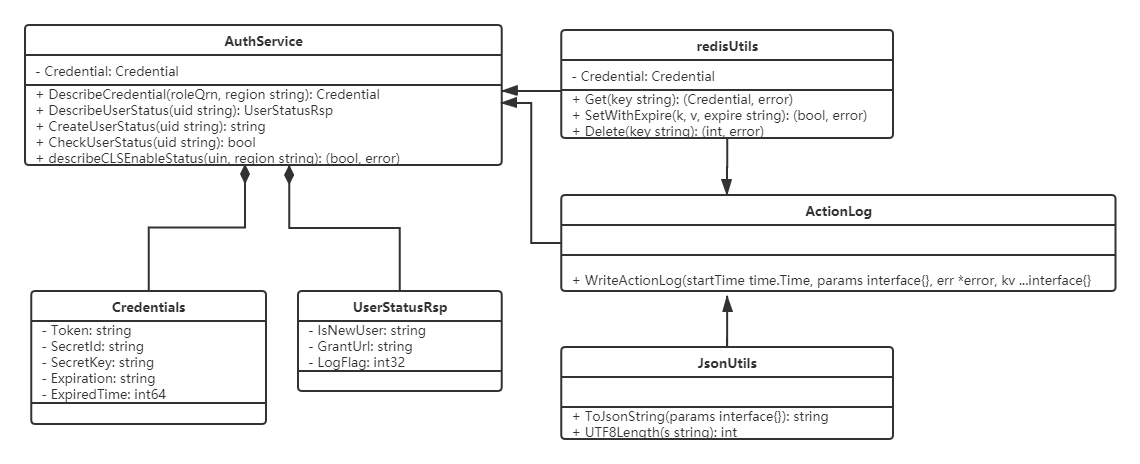
\includegraphics[width=1.0\textwidth]{class-auth.png}
        \caption{鉴权服务类图}
        \label{fig:jqfw}
    \end{figure}

    如图所示,AuthService负责提供权限权限秘钥申请、用户服务两大功能;通过增设缓存层,有限期地缓存用户申请到的Token,当到期时删除缓存,以保证不会
    频繁对服务器发送秘钥申请的请求,节约不必要的开销。

\subsubsection{接口设计}
CreateUserStatus:用户第一次使用该系统时,需要前端调用该接口为uid对应的用户创建一条数据,初始化该用户的状态和权限。
\begin{table}[H]
    \centering
    \caption{创建用户}
    \label{tab:design-interface-user-create}
    \begin{tabular}{llll}
        \toprule
        req, rsp   & 字段 & 类型 & 描述 \\
        \midrule
        req & uid & string & 用户id\\ \hline
        rsp & & & \\
        \bottomrule
    \end{tabular}
\end{table}

DescribeUserStatus:获取指定uid的用户当前状态,包括权限信息、日志投递标志信息。其中,日志投递位LogFlagBit是一个二进制数,目前仅
使用最低位和次低位。最低位为1则代表投递系统日志权限已开通,次低位为1则代表投递用户日志权限已开通。用户日志可供用户自己查看,也可用于
系统调试;而系统日志则仅用于内部调试以及数据收集与分析,不对外开放。
    \begin{table}[H]
        \centering
        \caption{获取用户状态}
        \label{tab:design-interface-user-status}
        \begin{tabular}{llll}
            \toprule
            req, rsp   & 字段 & 类型 & 描述 \\
            \midrule
            req &&& \\ \hline
            rsp & IsNewUser & bool & 是否新用户 \\
            & GrantUrl & string & 授权URL\\
            & LogFlagBit & int16 & 日志投递二进制标志位\\
            \bottomrule
        \end{tabular}
    \end{table}

    DescribeToken:该接口可以通过角色权限票据RoleQrn换取票据信息,所有模块的敏感操作都需要调用该接口,
以鉴别是否拥有该权限。如果该RoleQrn换取的是临时票据,则返回Token、SecretId、SecretKey以及过期时间;如果是永久票据,则返回
SecretId、SecretKey,其余字段为空。

    \begin{table}[H]
        \centering
        \caption{获取票据}
        \label{tab:design-interface-describe-token}
        \begin{tabular}{llll}
            \toprule
            req, rsp   & 字段 & 类型 & 描述 \\
            \midrule
            req & RoleQRN & string & 角色Qrn \\
            & Region & string & 用户所在地域 \\ \hline
            rsp & SecretId & string & 授权票据ID\\
            & SecretKey & string & 授权票据Key\\
            & Token & string & 临时票据Token,如果是临时票据,则非空\\
            & ExpiredTime & int64 & 临时票据过期时间,可空\\
            \bottomrule
        \end{tabular}
    \end{table}


\subsection{执行器微服务模块的设计与实现}

执行器模块的设计目标应是支持业务流量在不断增加的时候,执行器服务可以可靠地处理每一个用户提交的任务,通过弹性地进行容器的扩容和缩容,保持稳定的运行。

    \begin{figure}[H]
        \centering
        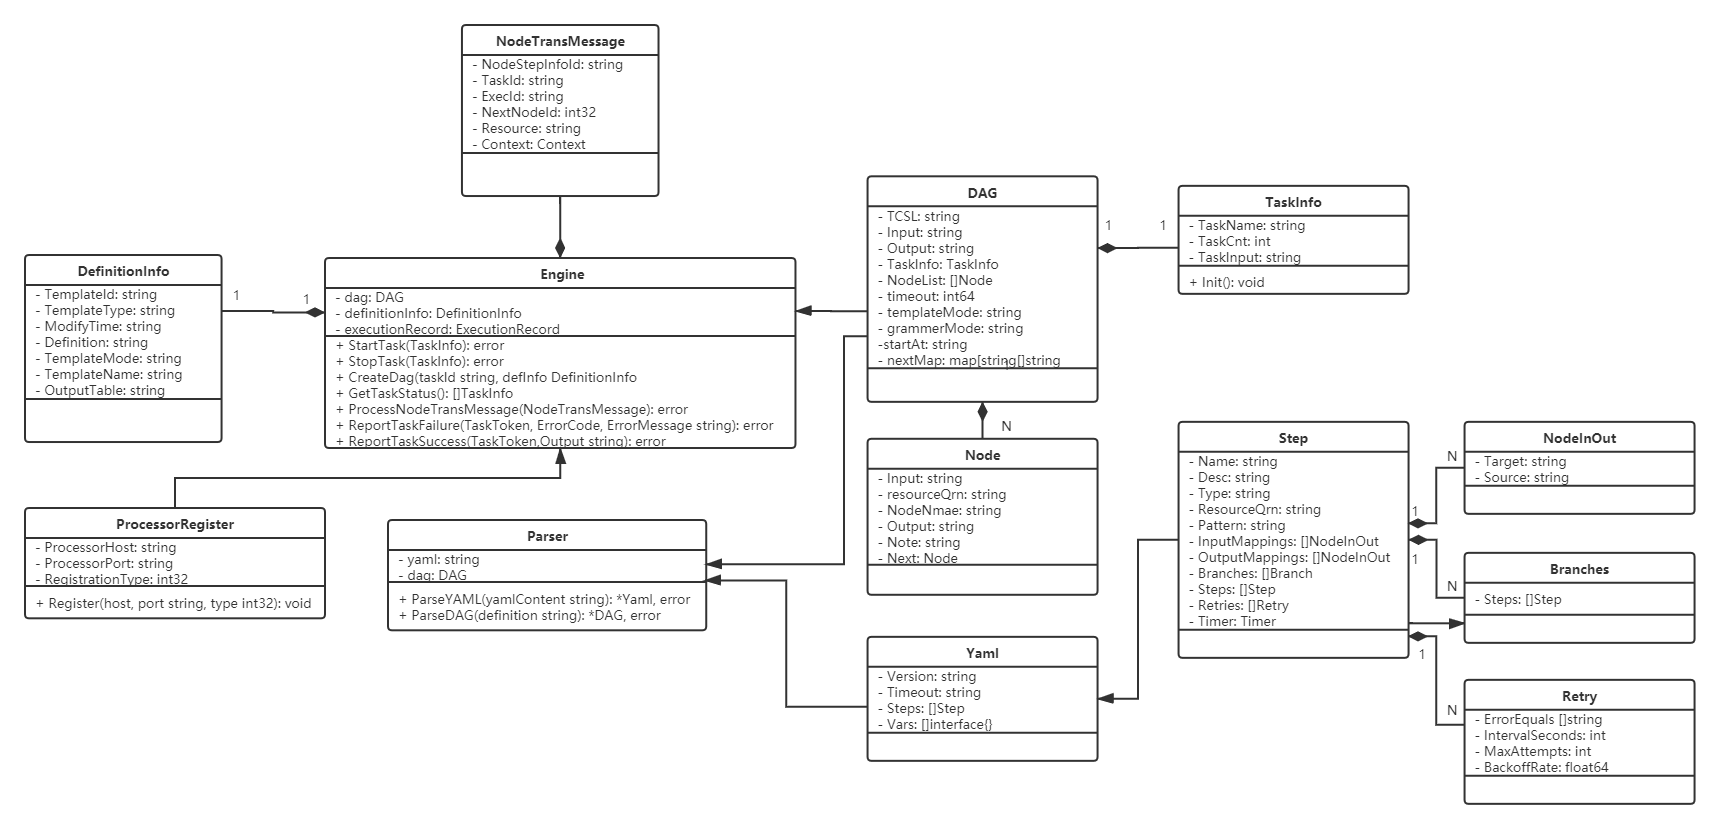
\includegraphics[width=1.0\textwidth]{class-processor.png}
        \caption{执行器服务类图}
        \label{fig:zxqfw}
    \end{figure}
    如图所示,将执行器划分为执行引擎、解析器、执行容器注册管理三个部分,由引擎负责执行用DAG来描述的任务;解析器则负责解析用户提交的工作流,生成DAG对象;
    ProcessorRegister负责提供容器的注册管理,心跳检查。


\begin{table}[H]
    \centering
    \caption{执行数据写入方案对比}
    \label{tab:design_1}
    \begin{tabular}{lp{12em}p{12em}l}
        \toprule
        & MySQL方案   & Redis + 云日志CLS方案          & 仅云日志CLS \\
        \midrule
        高并发能力 & 无 & Redis在流量过大时成为瓶颈 & 优秀\\
        复杂度 & 高, 大量数据写入消息队列
        大量消费者在处理数据
        大量数据写入MySQL(瓶颈)
        & 高, 大量数据写入消息队列;
        大量消费者处理消息队列中数据;
        大量数据写入Redis
        & 低\\
        支持现有所有功能 & 支持 & 支持 & 支持\\
        执行schema更新 & 支持 & 老数据无法更新 & 老数据无法更新\\
        成本 & 不变 & 包年付费 + 按量付费 & x\\
        技术扩展性 & 优秀,可使用Join语句 & 中等 & 中等\\
        容量扩展性 & 不可用 & 中等 & 优秀\\
        \bottomrule
    \end{tabular}
    \note{注:表}
\end{table}

接口设计:

SubmitCmd:该接口用于提交该任务ID对应的任务到容器节点,返回执行结果。调用方是调度器。当接收调度器提交的执行请求后,执行器负责通过
该接口调用解析器、执行引擎模块进行执行。

    \begin{table}[H]
        \centering
        \caption{提交执行}
        \label{tab:design-interface-submit-cmd}
        \begin{tabular}{llll}
            \toprule
            req, rsp   & 字段 & 类型 & 描述 \\
            \midrule
            req & Cmd & string & 命令内容,START=0; STOP=1; DROP=2; PAUSE=3\\
            & TaskInfo & Array & 任务集信息 \\
            & TaskId & string & 任务ID\\
            & Data & string & 任务输入\\
            & TaskMode & string & 任务模式\\
            & TaskType & string & 任务类型\\
            & Creator & string & 创建人\\
            & Operator & string & 执行人\\
            & ExecId & string & 代表该任务被执行的次数 \\ \hline
            rsp & ExecutionStatus & bool & 执行结果\\
            \bottomrule
        \end{tabular}
    \end{table}


    GetTaskStatus:执行器提供的接口,通过该接口可以获取执行器已提交的所有任务状态。

    \begin{table}[H]
        \centering
        \caption{获取当前执行任务的状态}
        \label{tab:design-interface-get-task-status}
        \begin{tabular}{llll}
            \toprule
            req, rsp   & 字段 & 类型 & 描述 \\
            \midrule
            req &  &  & \\ \hline
            rsp & TaskInfo & Array & 任务状态数组 \\
            & TaskInfo.TaskName & & 任务名称 \\
            & TaskInfo.TaskCnt & & 任务执行成功的节点数 \\
            & TaskInfo.TaskInput & & 任务输入 \\
            & TaskInfo.TaskOutput & & 任务输出 \\
            \bottomrule
        \end{tabular}
    \end{table}

Healthy:注册后的容器节点提供心跳检查的接口Healthy,调度器调用发至容器节点,即会返回该容器当前的负载情况以及任务执行状态。
    \begin{table}[H]
        \centering
        \caption{健康检查}
        \label{tab:design-interface-healthy}
        \begin{tabular}{llll}
            \toprule
            req, rsp   & 字段 & 类型 & 描述 \\
            \midrule
            req &&&\\ \hline
            rsp & Capacity & int32 & 负载值 \\
            & TaskHealthInfo & Array & 返回任务节点集的状态 \\
            & TaskHealthInfo.TaskId & string & 任务id。t\_scheduler\_task \\
            & TaskHealthInfo.TaskStatus & string & 任务状态 \\
            & TaskHealthInfo.TaskRuntimeStatus & string & 任务运行时状态 \\
            \bottomrule
        \end{tabular}
    \end{table}

\subsection{预测器微服务模块的设计与实现}


    \begin{figure}[H]
        \centering
        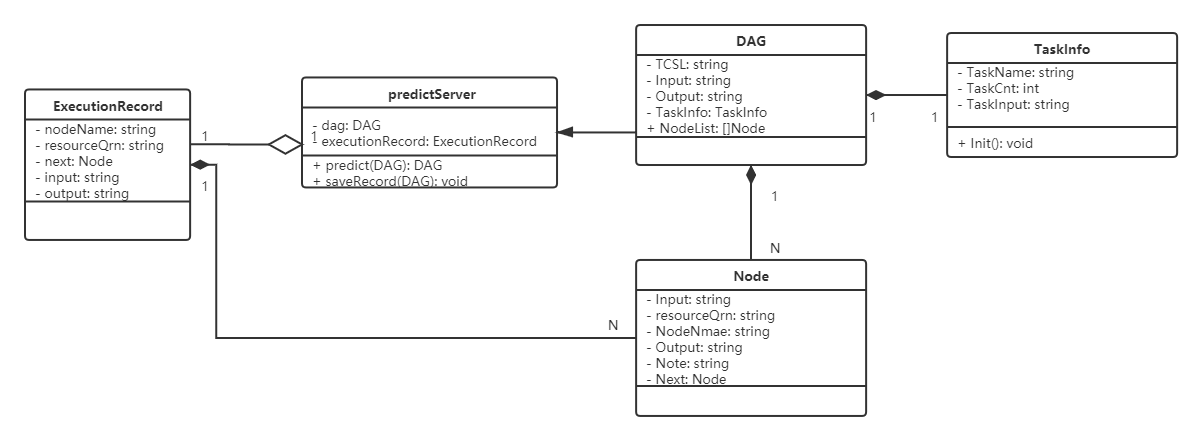
\includegraphics[width=1.0\textwidth]{class-predict.png}
        \caption{预测器服务类图}
        \label{fig:预测器服务类图}
    \end{figure}

    如图所示,预测器模块主要提供DAG输入输出预测,执行记录存储两大功能。预测器模块会将工作流的每次执行数据收集到数据库,预测器模块负责维护一个
    通过收集到的历史数据构成的哈希表缓存。在每次请求预测执行的时候,会通过缓存来查找对应的记录值,如果成功,则返回预测的结果;否则,根据预测执行模式
    来选择从数据库数据找到该预测值,或是取消本次预测请求,这会使得执行器直接退化为顺序执行模式进行后续节点的执行。


接口设计:

Predict:模块核心功能,提供对任务所有具有前置节点的节点的输入预测值,将所有预测值作为返回,如果ErrorCode非0,则代表此次执行无法进行
预测,或产生了非预期的错误,此时调用方(即执行器)将执行退化为顺序执行。
    \begin{table}[H]
        \centering
        \caption{获取预测值}
        \label{tab:design-interface-predict}
        \begin{tabular}{llll}
            \toprule
            req, rsp   & 字段 & 类型 & 描述 \\
            \midrule
            req & DAG & DAG & 待预测任务的有向无环图(DAG) \\ \hline
            rsp & DAG & DAG & 带有预测值的有向无环图(DAG) \\
            & ErrorCode & int & 错误代码 \\
            & ErrorMsg & string & 错误信息 \\
            \bottomrule
        \end{tabular}
    \end{table}

ExecutionRecord:将每次执行的任务输入输出对应起来并保存,为之后的执行提供预测服务时需要用到。输入是DAG
    \begin{table}[H]
        \centering
        \caption{执行记录提交}
        \label{tab:design-interface-execution-record}
        \begin{tabular}{llll}
            \toprule
            req, rsp   & 字段 & 类型 & 描述 \\
            \midrule
            req & DAG & DAG & 执行完毕的任务的有向无环图(DAG)\\ \hline
            rsp & & & \\
            \bottomrule
        \end{tabular}
    \end{table}

以上接口设计所用到的复杂结构体如下:
    \begin{table}[H]
        \centering
        \caption{复杂结构体定义}
        \label{tab:design-interface-struct-definition}
        \begin{tabular}{llll}
            \toprule
            结构体名称& 字段 & 类型 & 描述 \\
            \midrule
            DAG & TCSL & string & 该任务的TCSL定义 \\
                & Input & string & 节点执行输入 \\
                & Output & string & 节点执行输出 \\
                & TaskInfo & TaskInfo & 保存任务信息 \\
                & NodeList & []Node & 后续节点数组 \\ \hline
            TaskInfo    & TaskName & string & 任务名称 \\
                        & TaskCnt & int & 任务执行节点数量 \\
                        & TaskInput & string & 任务执行输入 \\ \hline
            Node    & Input & TaskInfo & 节点输入 \\
                    & Output & string & 节点输出 \\
                    & NodeName & string & 任务名称 \\
                    & ResourceQrn & string & 资源Qrn \\
                    & Note & string & 节点说明 \\
                    & Next & Node & 后续节点 \\

            \bottomrule
        \end{tabular}
    \end{table}


\section{数据库}
由于业务数据持久化的需要,以MySQL作为主要业务数据库,存储用户数据、工作流状态数据、容器状态管理等。

\subsection{表设计}

模板表t\_flow\_template:存储模板相关信息,可通过id作为索引项快速找到一个模板,记录该模板定制后的状态,一般不对原有模板进行频繁修改,
以读取操作占多数,因此,设计时应确保足够的索引项,方便提高查找时效率。
\begin{table}[H]
    \centering
    \caption{模板表}
    \label{tab:t_flow_template}
    \begin{tabular}{lllllll}
        \toprule
        字段名	&类型	&长度	&可为Null	&键	&默认值	&描述 \\
        \midrule
        f\_id	&int	&11 &&&& \\
        f\_template\_id	&varchar	&20 &&&& \\
        f\_service\_id	&varchar	&20 &&&& \\
        f\_category	&varchar	&12 &&&& \\
        f\_status	&varchar	&64 &&&& \\
        f\_create\_time	&timestamp & &&&& \\
        f\_modify\_time   &timestamp & &&&& \\
        f\_creator	&varchar	&64 &&&& \\
        f\_modifier	&varchar	&64 &&&& \\
        f\_app\_id	&int	&18 &&&& \\
        \bottomrule
    \end{tabular}
    \note{注:1}
\end{table}

执行器表t\_processor:存储现有的资源机器,作为调度器进行资源编排和负载均衡的依据。
\begin{table}[H]
    \centering
    \caption{执行器表}
    \label{tab:t_processor}
    \begin{tabular}{lllllll}
        \toprule
        字段名	&类型	&长度	&可为Null	&键	&默认值	&描述 \\
        \midrule
        f\_id	&int	&11 &&&& \\
        f\_processor\_host	&varchar	&20 &&&& \\
        f\_processor\_port	&varchar	&20 &&&& \\
        f\_processor\_load	&int	&11 &&&& \\
        f\_last\_hearbeat\_time	&datetime & &&&& \\
        f\_status	&int	&11 &&&& \\
        f\_registration\_time	&datetime & &&&& \\
        f\_logout\_time	&datetime & &&&& \\
        f\_logout\_reason	&int	&11 &&&& \\
        \bottomrule
    \end{tabular}
    \note{注:1}
\end{table}

工作流服务表t\_flow\_service:以服务对象作为单位,将该对象称作工作流,表设计应将服务id、模板id存储为一条记录,互相关联。
\begin{table}[H]
    \centering
    \caption{工作流服务表}
    \label{tab:t_flow_service}
    \begin{tabular}{lllllll}
        \toprule
        字段名	&类型	&长度	&可为Null	&键	&默认值	&描述 \\
        \midrule
        f\_id	&bigint	&20 &&&& \\
        f\_service\_id	&varchar	&64 &&&& \\
        f\_machine\_qrn	&varchar	&128 &&&& \\
        f\_role\_qrn	&varchar	&128 &&&& \\
        f\_template\_id	&varchar	&64 &&&& \\
        f\_switch\_bit	&tinyint	&4 &&&& \\
        f\_service\_name	&varchar	&64 &&&& \\
        f\_machine\_type	&varchar	&64 &&&& \\
        f\_category	&varchar	&12 &&&& \\
        f\_status	&varchar	&64 &&&& \\
        f\_create\_time	&timestamp & &&&& \\
        f\_modify\_time   &timestamp & &&&& \\
        f\_creator	&varchar	&64 &&&& \\
        f\_modifier	&varchar	&64 &&&& \\
        f\_app\_id	&int	&18 &&&& \\
        \bottomrule
    \end{tabular}
    \note{注:表注分两种,第一种是对全表的注释,用不加阿拉伯数字排在表的下边,
    前面加“注:”;第二种是和表内的某处文字或数字相呼应的注,
    在表里面用带圈的阿拉伯数字在右上角标出,然后在表下面用同样的圈码注出来}
\end{table}

工作流调度记录表t\_execution:模拟操作系统调度任务操作,将每个任务抽象为一个整体,存储该任务的上下文信息,方便运行时存储任务状态,
模拟TCB的各项数据存储,将其存储为一个表,为方便定位每一个当前任务,索引应设置任务ID。
\begin{table}[H]
    \centering
    \caption{执行器表}
    \label{tab:t_execution}
    \begin{tabular}{lllllll}
        \toprule
        字段名	&类型	&长度	&可为Null	&键	&默认值	&描述 \\
        \midrule
        f\_id	&bigint	&20 &否 & & &主键 \\
        f\_service\_id	&varchar	&64 &否 & & &工作流id \\
        f\_machine\_qrn	&varchar	&128 &否 & & &物理机器QRN \\
        f\_execution\_name	&varchar	&128 &否 & & &该次执行名称 \\
        f\_execution\_qrn	&varchar	&128 &否 & & &该次执行QRN \\
        f\_execution\_definition	&text	& &否 & & &工作流的模板TCSL定义 \\
        f\_start\_time	&varchar	&20 &否 & & &执行开始时间 \\
        f\_end\_time	&varchar	&20 &否 & & &执行结束时间 \\
        f\_execution\_status	&varchar	&20 &否 & & &当前执行状态,枚举值Success, Failed, Running, Pause \\
        f\_input	&text	& &否 & & &工作流的用户输入 \\
        f\_output	&text	& &否 & & &工作流执行的输出 \\
        f\_processor\_id	&int	&11 &否 & & &执行物理机器的id \\
        \bottomrule
    \end{tabular}
    \note{注:}
\end{table}


template\_resource表t\_template\_execution:负责记录工作流应用模板所需要的所有外部资源
\begin{table}[H]
    \centering
    \caption{模板资源表}
    \label{tab:t_template_resource}
    \begin{tabular}{lllllll}
        \toprule
        字段名	&类型	&长度	&可为Null	&键	&默认值	&描述 \\
        \midrule
        f\_id	&bigint	&20 &否 &&& 主键id\\
        f\_type	&varchar	&255 &否 &&& 资源类型\\
        f\_template\_id	&varchar	&64 &否 &&& 模板id\\
        f\_name	&varchar	&255 &否 &&& 应用模板名称\\
        f\_description	&varchar	&255 &否 &&& 应用模板描述\\
        f\_event\_node\_name	&varchar	&255 &否 &&& 在工作流中的节点名称\\
        f\_service\_url	&varchar	&255 &否 &&& 外部服务的控制台地址\\
        f\_describe\_status\_url	&varchar	&255 &否 &&& 查询外部服务的url\\
        f\_status	&tinyint	&4 &否 &&& 可用状态,0, 1枚举值\\
        f\_create\_time	&timestamp	& &否 &&CURRENT\_TIMESTAMP & 创建时间\\
        f\_last\_update\_time	&timestamp	& &否 &&CURRENT\_TIMESTAMP & 最后一次更新时间\\
        \bottomrule
    \end{tabular}
    \note{注:}
\end{table}

t\_user表t\_user:负责记录用户鉴权信息
\begin{table}[H]
    \centering
    \caption{用户表}
    \label{tab:t_user}
    \begin{tabular}{lllllll}
        \toprule
        字段名	&类型	&长度	&可为Null	&键	&默认值	&描述 \\
        \midrule
        f\_id	&bigint	&20 &否 &&& 主键id\\
        f\_uin	&varchar	&128 &否 &&& 用户uin\\
        f\_app\_id	&varchar	&128 &否 &&& 用户appId\\
        f\_status	&varchar	&20 &否 &&& 用户状态\\
        f\_create\_time	&datetime	& &否 &&CURRENT\_TIMESTAMP  & 创建时间\\
        f\_last\_login\_time	&datetime	& &否 &&CURRENT\_TIMESTAMP  & 最后一次登录时间\\
        f\_cls\_logset\_id	&varchar	&255 &否 &&& 日志集id\\
        f\_cls\_topic\_id	&varchar	&255 &否 &&& 日志主题id\\
        f\_log\_bit	&tinyint	&4 &否 &&& 日志授权标志二进制位, 高位1:需要写入用户提供的日志集,低位1:需要写入系统提供的日志集\\
        \bottomrule
    \end{tabular}
    \note{注:}
\end{table}
\subsection{表设计}

\section{缓存}
由于每个模块承受处理的流量不一致,存在性能瓶颈模块。针对该部分需要设计基于缓存的存储方案,实现对服务高性能、可用性和稳定性的保障。



使用REDIS 的sorted set存储最近的N个Execution数据 (双写redis方案)

插入:
元数据O(1):
HSET E\_\{StateMachineQRN\}\_\{ExecutionQRN\} metadata $\{execution details\}, status $\{status\}, output $\{output\} StopDate $\{1238192837\}

列表数据O(1):
ZADD Executions\_\{StateMachineQRN\} \$\{current\_timestamp\} \$\{name, status, start\_time, end\_time\}
Execution对应的stateMachine信息 O(1):
set $\{ExecutionQRN\} $\{stateMachineQRN\}

分页查询:
查询zset数据O(logN + M): ZRANGE key start stop
zcount查询总条数 ZCOUNT key min max

单条查询O(1):
HGET  EXECUTION\_\{MachineQRN\}\_\{ExecutionQRN\}

判断是否存在 O(1):
HEXISTS EXECUTION\_\{MachineQRN\}\_\{ExecutionQRN\}

更新:
HSET EXECUTION\_\{MachineQRN\}\_\{ExecutionQRN\} data \{execution\_details\}
采用LRU淘汰策略清理数据:

获取待清理数据: ZRANGE key min max [LIMIT offset count]

清理ZSet列表数据: ZREMRANGE key min max

遍历找到的所有Key:

使用HDEL删除元数据

使用DEL删除Execution对应的stateMachine信息



\subsection{键设计}
由于用户查询执行记录是高频操作,因此需要单独存储到ZSet,使其可以根据时间排序,作为读取这些记录时的缓存,并且通过定时清理过期数据,
保证内存使用量在可控范围以内。

在原系统中,有很多操作是依赖于关系型数据库查询语句来实现的查询,在将执行记录表迁移到Redis后,必须将这些业务查询逻辑进行等效替换。
方案是以空间换时间,通过额外的哈希表和字符串键值对,将MachineQrn映射到ExecutionQrn,再通过ExecutionQrn从哈希表找到该执行Qrn对应的
工作流执行记录详情。

综上,即缓存部分包含执行日志列表、执行日志详情、执行日志索引三个部分,存储的内容是相似的,但查询方式是不同的。
其中,执行日志详情存储所有的信息,Metadata存储不可变的数据,一次写入之后不进行修改,其余字段是可变数据,写入后可进行修改;
执行日志列表只存储列表页面查询时显示的数据;而索引则用于通过资源定位符MachineQrn查询到对应此次执行时执行器生成的ExecutionQrn,
进一步地,可以根据ExecutionQrn来查询到执行记录详情。这样一来,就通过增加空间开销的代价,实现了所有关系型数据库时需要实现的所有操作。

    \begin{table}[H]
        \centering
        \caption{执行日志列表}
        \label{tab:key-log-list}
        \begin{tabular}{lp{10em}ll}
            \toprule
            对象   & 数据               & 说明 & Key格式 \\
            \midrule
            日志列表     & MachineQrn    & 机器QRN                    & ES\_\$\{MachineQrn\} \\
            & ExecutionQrn  & Unix时间戳, 单位:微秒 &\\
            & Output        & 输出 &\\
            & Status        & 状态 &\\
            & EndTime       & 终止时间 &\\
            \bottomrule
        \end{tabular}
    \end{table}



    \begin{table}[H]
        \centering
        \caption{执行日志详情}
        \label{tab:key-log-hash}
        \begin{tabular}{lp{8em}ll}
            \toprule
            对象   & 数据               & 说明 & Key格式 \\
            \midrule
            日志详细信息 & MachineQrn    & 机器QRN                      & E\_\$\{MachineQrn\}\_\$\{ExecutionQrn\}\\
            (HashTable) & ExecutionQrn  & 执行QRN &\\
            & Metadata      & 不可变数据部分(JSON)&\\
            & Status        & 状态,需要频繁更新的字段 &\\
            & Output        & 输出,需要频繁更新的字段 &\\
            & EndTime       & 终止时间,需要频繁更新的字段 &\\
            \bottomrule
        \end{tabular}
        \note{注:}
    \end{table}

    \begin{table}[H]
        \centering
        \caption{执行日志索引}
        \label{tab:key-log-index}
        \begin{tabular}{lp{10em}ll}
            \toprule
            对象   & 数据               & 说明 & Key格式 \\
            \midrule
            ExecutionQrn索引 & ExecutionQrn    & 执行QRN    & E\_\$\{MachineQrn\} \\
            (string) &&& \\
            \bottomrule
        \end{tabular}
        \note{注:}
    \end{table}

\subsection{查询合并}
3个表越权检查、工作流表、模板表查询可以合并为一个join查询
只查询需要的字段, 其他无用字段不写入select中, 优化网络流量


\section{本章小结}
本章的工作在第四章的概要设计的基础上,详细的阐述了系统重构方案的具体实现。基于上一章提出的设计方案,通过对代码的重构,中间件的替换和
缓存层的引入等方式,将系统整体的运行效率提升了数个档次,使得能够在大流量的场景下保持服务的可用性